\documentclass[12pt]{article}

% Codificación y lenguaje
\usepackage[utf8]{inputenc}
\usepackage[T1]{fontenc}
\usepackage[spanish]{babel}
\usepackage{tikz}
\usetikzlibrary{positioning, arrows.meta}
\usepackage{graphicx}
\usepackage{tabularx}
\usepackage{hyperref}
\usepackage{amsmath}

% Márgenes
\usepackage[a4paper, left=2.5cm, right=2.5cm, top=2cm, bottom=2cm]{geometry}

% Gráficos, flotantes y código
\usepackage{graphicx}
\usepackage{caption}
\usepackage{float}
\usepackage{listings}
\usepackage{xcolor}
\usepackage{tikz}
\usepackage{url}

% Encabezados y pies de página
\usepackage{fancyhdr}
\pagestyle{fancy}
\fancyhf{}
\lhead{TP Final - Cancelación Adaptiva de Ruido}
\rhead{UNC-Procesamiento digital de señales}
\cfoot{\thepage}
\setlength{\headheight}{15pt}

% Estilo para código
\definecolor{codegreen}{rgb}{0,0.6,0}
\definecolor{codegray}{rgb}{0.5,0.5,0.5}
\definecolor{codepurple}{rgb}{0.58,0,0.82}
\definecolor{backcolour}{rgb}{0.95,0.95,0.92}

\lstdefinestyle{mystyle}{
	language=C,
	backgroundcolor=\color{white},
	basicstyle=\scriptsize\ttfamily,
	keywordstyle=\color[HTML]{0072BD}\bfseries,
	commentstyle=\color[HTML]{008000}\itshape,
	stringstyle=\color[HTML]{A2142F},
	numberstyle=\tiny\color{gray},
	numbers=left,
	numbersep=6pt,
	frame=single,
	rulecolor=\color{black!50},
	breaklines=true,
	breakatwhitespace=false,
	breakautoindent=true,
	tabsize=2,
	showspaces=false,
	showstringspaces=false,
	xleftmargin=1.5em,
	xrightmargin=0.5em,
	aboveskip=1em,
	belowskip=1em,
	literate={á}{{\'a}}1 {é}{{\'e}}1 {í}{{\'\i}}1 {ó}{{\'o}}1 {ú}{{\'u}}1 {ñ}{{\~n}}1 {Á}{{\'A}}1 {É}{{\'E}}1 {Í}{{\'I}}1 {Ó}{{\'O}}1 {Ú}{{\'U}}1 {Ñ}{{\~N}}1 {≈}{{$\approx$}}1,
}

\lstdefinestyle{pythonstyle}{
	language=Python,
	backgroundcolor=\color{white},
	basicstyle=\scriptsize\ttfamily,
	keywordstyle=\color[HTML]{0000FF}\bfseries,
	commentstyle=\color[HTML]{008000}\itshape,
	stringstyle=\color[HTML]{A2142F},
	numberstyle=\tiny\color{gray},
	numbers=left,
	numbersep=6pt,
	frame=single,
	rulecolor=\color{black!50},
	breaklines=true,
	breakatwhitespace=false,
	breakautoindent=true,
	tabsize=4,
	showspaces=false,
	showstringspaces=false,
	xleftmargin=1.5em,
	xrightmargin=0.5em,
	aboveskip=1em,
	belowskip=1em,
	literate={á}{{\'a}}1 {é}{{\'e}}1 {í}{{\'\i}}1 {ó}{{\'o}}1 {ú}{{\'u}}1 {ñ}{{\~n}}1 {Á}{{\'A}}1 {É}{{\'E}}1 {Í}{{\'I}}1 {Ó}{{\'O}}1 {Ú}{{\'U}}1 {Ñ}{{\~N}}1 {≈}{{$\approx$}}1,
}

% Título y autores
\title{
	
\includegraphics[width=0.45\textwidth]{unc.png} \\[2cm] % Logo
	\textbf{Trabajo Práctico Final: Acondicionamiento de señal SG} 
}
    
\author{
	Profesores: \\ Parlanti Gustavo Fernand (Presidente) \\ Molina German Alcides (Vocal)\\ Rossi Robreto Raul (Vocal)
	\\ \\
	Alumnos:\\ Campos \\ Testa \\ Verstraete 
}

\date{Junio de 2026} % Fecha del trabajo

\begin{document}
	
	\maketitle
	
	\begin{abstract}
	En este trabajo práctico se implementa el algoritmo de Pan--Tompkins sobre la plataforma STM32F446RE para la detección automática de complejos QRS en señales electrocardiográficas (ECG). El sistema realiza la adquisición de la señal, su procesamiento en tiempo real mediante la biblioteca CMSIS-DSP y la visualización de las distintas etapas del algoritmo utilizando los periféricos del microcontrolador. Finalmente, se evalúa el funcionamiento del sistema mediante ensayos experimentales, verificando la correcta ejecución de cada etapa del procesamiento y la detección de los complejos QRS.
	\end{abstract} 
	\newpage
	
	\tableofcontents \newpage
	
	\section{Introducción}

		El procesamiento digital de señales biomédicas constituye una de las aplicaciones más relevantes del procesamiento digital de señales (DSP), ya que permite extraer información de interés a partir de registros fisiológicos adquiridos mediante sensores electrónicos. Entre estas señales, el electrocardiograma (ECG) ocupa un lugar destacado debido a que proporciona información sobre la actividad eléctrica del corazón, siendo ampliamente utilizado para el monitoreo de pacientes, el diagnóstico de patologías cardíacas y la estimación de parámetros fisiológicos como la frecuencia cardíaca.

		Una de las tareas fundamentales en el análisis automático de señales ECG consiste en la detección de los complejos QRS, ya que estos representan la despolarización de los ventrículos y permiten determinar con precisión el instante en que ocurre cada latido cardíaco. Sin embargo, la presencia de ruido producido por el movimiento del paciente, interferencias de la red eléctrica y actividad muscular dificulta la detección directa de dichos complejos, haciendo necesario el empleo de técnicas de procesamiento digital que permitan mejorar la relación señal-ruido antes de realizar su identificación.

		Entre los algoritmos desarrollados para este propósito, el método propuesto por Pan y Tompkins constituye una de las soluciones más difundidas debido a su robustez, bajo costo computacional y facilidad de implementación en sistemas embebidos. El algoritmo se basa en una secuencia de etapas de procesamiento que incluyen filtrado pasa banda, derivación, elevación al cuadrado e integración mediante una ventana móvil, con el objetivo de resaltar las características temporales asociadas al complejo QRS y detectar automáticamente los latidos cardíacos mediante un esquema de umbrales adaptativos.

		En este trabajo práctico se implementará el algoritmo de Pan--Tompkins sobre la plataforma de desarrollo STM32F446RE, continuando con la arquitectura de adquisición y procesamiento en tiempo real desarrollada en los laboratorios anteriores. La señal ECG será adquirida mediante los convertidores analógico-digitales (ADC) del microcontrolador y procesada utilizando la biblioteca CMSIS-DSP. La salida correspondiente a la señal procesada para la detección de complejos QRS será transmitida por uno de los canales del convertidor digital-analógico (DAC), mientras que el segundo canal permitirá visualizar, mediante la selección realizada con un pulsador, tanto la señal de entrada como las salidas intermedias de las distintas etapas del algoritmo.

		El presente documento describe los fundamentos teóricos del algoritmo de Pan--Tompkins, el diseño e implementación del sistema sobre la plataforma STM32, la configuración de los periféricos utilizados, la implementación de cada una de las etapas de procesamiento digital, el esquema de detección mediante umbrales adaptativos y los resultados experimentales obtenidos durante la validación del sistema en tiempo real.

		\subsection{Objetivos del proyecto}

			\begin{itemize}

			\item Implementar el algoritmo de Pan--Tompkins sobre el microcontrolador STM32F446RE para el procesamiento en tiempo real de señales electrocardiográficas.

			\item Implementar las etapas de filtrado pasa banda, derivación, elevación al cuadrado e integración por ventana móvil que conforman el algoritmo de Pan--Tompkins.

			\item Implementar un algoritmo de detección de complejos QRS basado en umbrales adaptativos sobre la señal resultante del preprocesamiento.

			\item Utilizar la biblioteca CMSIS-DSP para optimizar la ejecución de las etapas de procesamiento digital sobre la arquitectura ARM Cortex-M4.

			\item Visualizar mediante el convertidor digital-analógico (DAC) tanto la señal procesada para la detección de complejos QRS como las salidas intermedias de cada etapa del algoritmo, seleccionables mediante un pulsador.

			\item Implementar una arquitectura de procesamiento en tiempo real basada en ADC, DAC, DMA y temporizadores, garantizando un flujo continuo de adquisición y procesamiento de datos.

			\item Evaluar experimentalmente el desempeño del algoritmo implementado, verificando el funcionamiento de cada etapa del procesamiento y la correcta detección de los complejos QRS.

			\end{itemize}
			
	\section{Marco teórico}

		La implementación de algoritmos de procesamiento digital de señales biomédicas en sistemas embebidos requiere comprender tanto las características fisiológicas de las señales involucradas como las técnicas digitales empleadas para su análisis. En particular, la detección automática de complejos QRS en señales electrocardiográficas constituye un problema clásico del procesamiento digital de señales, ya que combina etapas de filtrado, análisis temporal y toma de decisiones sobre señales adquiridas en tiempo real.

		En esta sección se presentan los fundamentos teóricos necesarios para comprender el funcionamiento del algoritmo de Pan--Tompkins y su implementación sobre la plataforma STM32F446RE. En primer lugar se describen las principales características del electrocardiograma y la información fisiológica contenida en sus diferentes componentes. Posteriormente se desarrollan las etapas que conforman el algoritmo de Pan--Tompkins, incluyendo el filtrado pasa banda, la etapa derivativa, la operación de elevación al cuadrado, la integración mediante ventana móvil y el mecanismo de detección basado en umbrales adaptativos. Finalmente, se introducen las consideraciones necesarias para su implementación en tiempo real sobre sistemas embebidos utilizando la biblioteca CMSIS-DSP.
		
			\subsection{Electrocardiograma (ECG)}

				El electrocardiograma (ECG) es una señal biomédica que representa la actividad eléctrica del corazón en función del tiempo. Esta señal se obtiene mediante electrodos colocados sobre la superficie del cuerpo, los cuales registran las pequeñas diferencias de potencial generadas por los procesos de despolarización y repolarización del tejido cardíaco. Debido a que estas variaciones eléctricas son de baja amplitud y pueden estar afectadas por ruido externo o interferencias fisiológicas, su análisis requiere etapas de acondicionamiento y procesamiento digital adecuadas.

				Desde el punto de vista del procesamiento digital de señales, el ECG puede considerarse una señal temporal de baja frecuencia, no estacionaria y de morfología repetitiva. Cada ciclo cardíaco está compuesto por una serie de ondas características que permiten identificar las distintas fases de activación eléctrica del corazón. En condiciones normales, estas componentes se repiten de manera periódica o cuasi periódica, aunque su forma, amplitud y duración pueden variar según el paciente, el estado fisiológico y las condiciones de adquisición.

				\subsubsection{Actividad eléctrica del corazón}

				El funcionamiento mecánico del corazón está gobernado por impulsos eléctricos que se propagan a través del sistema de conducción cardíaco. Estos impulsos producen la contracción coordinada de las aurículas y los ventrículos, permitiendo el bombeo de sangre hacia el resto del organismo. La señal ECG es, por lo tanto, una representación indirecta de esta actividad eléctrica medida desde la superficie corporal.

				Durante cada latido, la activación eléctrica comienza normalmente en el nodo sinoauricular, se propaga por las aurículas, atraviesa el nodo auriculoventricular y finalmente se distribuye por los ventrículos a través del haz de His y las fibras de Purkinje. Este proceso genera cambios de potencial que pueden ser registrados externamente y que dan origen a las distintas ondas visibles en el ECG.

				\subsubsection{Ondas características del ECG}

				Una señal ECG típica está formada principalmente por la onda P, el complejo QRS y la onda T. Cada una de estas componentes está asociada a una etapa específica del ciclo eléctrico cardíaco.

				La onda P representa la despolarización de las aurículas. Esta componente suele tener una amplitud reducida y una variación temporal relativamente lenta en comparación con el complejo QRS. Su presencia indica el inicio de la activación eléctrica que precede a la contracción auricular.

				El complejo QRS corresponde a la despolarización de los ventrículos. Es la componente más prominente de la señal ECG debido a la mayor masa muscular ventricular y a la velocidad con la que ocurre este proceso de activación. Desde el punto de vista temporal, el complejo QRS presenta pendientes pronunciadas y una duración reducida, lo que lo convierte en la característica más adecuada para detectar el instante de ocurrencia de cada latido cardíaco.

				La onda T representa la repolarización de los ventrículos, es decir, el proceso mediante el cual el tejido ventricular recupera su estado eléctrico previo para prepararse para el siguiente ciclo cardíaco. Esta onda suele ser más ancha y de menor pendiente que el complejo QRS, por lo que posee un contenido frecuencial más bajo.

				\begin{figure}[H]
				\centering
				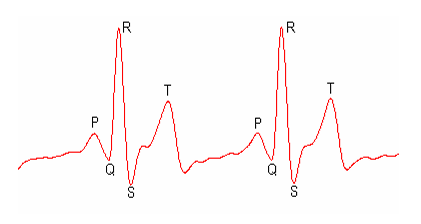
\includegraphics[width=0.7\textwidth]{imagenes/QRS_signal.png}
				\caption{Señal típica de un electrocardiograma (ECG).}
				\label{fig:ecg}
				\end{figure}

				\subsubsection{Complejo QRS y frecuencia cardíaca}

				La detección del complejo QRS es una etapa fundamental en el análisis automático de señales ECG, ya que permite identificar los instantes en los que ocurren los latidos cardíacos. A partir de estos instantes puede calcularse el intervalo RR, definido como el tiempo transcurrido entre dos complejos QRS consecutivos.

				Si el intervalo RR se expresa en segundos, la frecuencia cardíaca puede estimarse mediante:

				\begin{equation}
					FC = \frac{60}{T_{RR}}
				\end{equation}

				donde $FC$ es la frecuencia cardíaca expresada en latidos por minuto y $T_{RR}$ es el intervalo temporal entre dos picos R consecutivos.

				En una señal ECG ideal, la detección del complejo QRS podría realizarse simplemente localizando los máximos de amplitud. Sin embargo, en señales reales esto no resulta suficiente, ya que pueden aparecer interferencias de baja frecuencia, ruido muscular, ruido de red eléctrica, variaciones de línea base y cambios de amplitud entre distintos latidos. Por esta razón, los algoritmos de detección suelen incorporar etapas de filtrado y realce de características antes de aplicar un criterio de decisión.

				\subsubsection{Contenido frecuencial de la señal ECG}

				La señal ECG presenta componentes espectrales distribuidas principalmente en bajas frecuencias. Las variaciones lentas, como la línea base y las ondas P y T, se encuentran asociadas a componentes de menor frecuencia, mientras que el complejo QRS contiene componentes de frecuencia más altas debido a sus pendientes pronunciadas y corta duración temporal.

				Esta diferencia en el contenido espectral permite aplicar técnicas de filtrado digital para atenuar componentes no deseadas y resaltar la información asociada al complejo QRS. En particular, el algoritmo de Pan--Tompkins utiliza una etapa de filtrado pasa banda para reducir tanto las componentes de muy baja frecuencia, asociadas a desplazamientos de línea base o movimientos, como las componentes de alta frecuencia, asociadas a ruido muscular o interferencias externas.

				De esta manera, el conocimiento de la morfología y del contenido frecuencial del ECG resulta fundamental para comprender el diseño de los algoritmos de detección automática de latidos. El complejo QRS, por su amplitud relativa, pendiente elevada y duración reducida, constituye la característica principal utilizada por el algoritmo de Pan--Tompkins para realizar la detección de eventos cardíacos en tiempo real.

			\subsection{Algoritmo de Pan--Tompkins}

				El algoritmo de Pan--Tompkins, propuesto por Jiapu Pan y Willis J. Tompkins en 1985, constituye uno de los métodos más utilizados para la detección automática de complejos QRS en señales electrocardiográficas. Su amplia difusión se debe a su elevada precisión, bajo costo computacional y facilidad de implementación en sistemas de procesamiento digital en tiempo real, características que lo convierten en una alternativa adecuada para aplicaciones embebidas y dispositivos portátiles de monitoreo cardíaco.

				El objetivo principal del algoritmo es determinar con precisión el instante de ocurrencia de cada latido cardíaco a partir de una señal ECG adquirida en tiempo real. Para ello, la señal es sometida a una serie de etapas de procesamiento digital que permiten eliminar ruido, resaltar las características del complejo QRS y facilitar su identificación mediante un criterio de decisión basado en umbrales adaptativos.

				A diferencia de otros métodos que realizan la detección directamente sobre la señal ECG original, el algoritmo de Pan--Tompkins transforma progresivamente la señal hasta obtener una representación en la cual los complejos QRS aparecen claramente diferenciados del resto de las componentes del electrocardiograma y de las interferencias presentes durante la adquisición. Esta estrategia mejora significativamente la robustez del algoritmo frente a variaciones de amplitud, ruido muscular, desplazamientos de la línea base e interferencias producidas por la red eléctrica.

				El procesamiento puede dividirse en dos grandes etapas. La primera corresponde al preprocesamiento de la señal, donde se aplican sucesivamente un filtro pasa banda, un operador derivativo, una operación de elevación al cuadrado y una integración mediante ventana móvil. Estas operaciones permiten realzar las pendientes características del complejo QRS y reducir la influencia de componentes no deseadas presentes en la señal.

				La segunda etapa corresponde al proceso de decisión, en el cual la señal integrada es analizada mediante un conjunto de umbrales adaptativos que se actualizan dinámicamente de acuerdo con la amplitud de los complejos detectados y el nivel de ruido presente en la señal. De esta manera, el algoritmo es capaz de distinguir entre verdaderos complejos QRS y falsas detecciones ocasionadas por interferencias o artefactos.

				La Figura \ref{fig:pan_tompkins} muestra el diagrama en bloques simplificado del algoritmo de Pan--Tompkins. Puede observarse que la señal ECG atraviesa sucesivamente las distintas etapas de procesamiento hasta obtener una señal acondicionada para la detección de los complejos QRS. Cada uno de estos bloques será analizado con mayor detalle en las siguientes secciones.

				\begin{figure}[H]
					\centering
					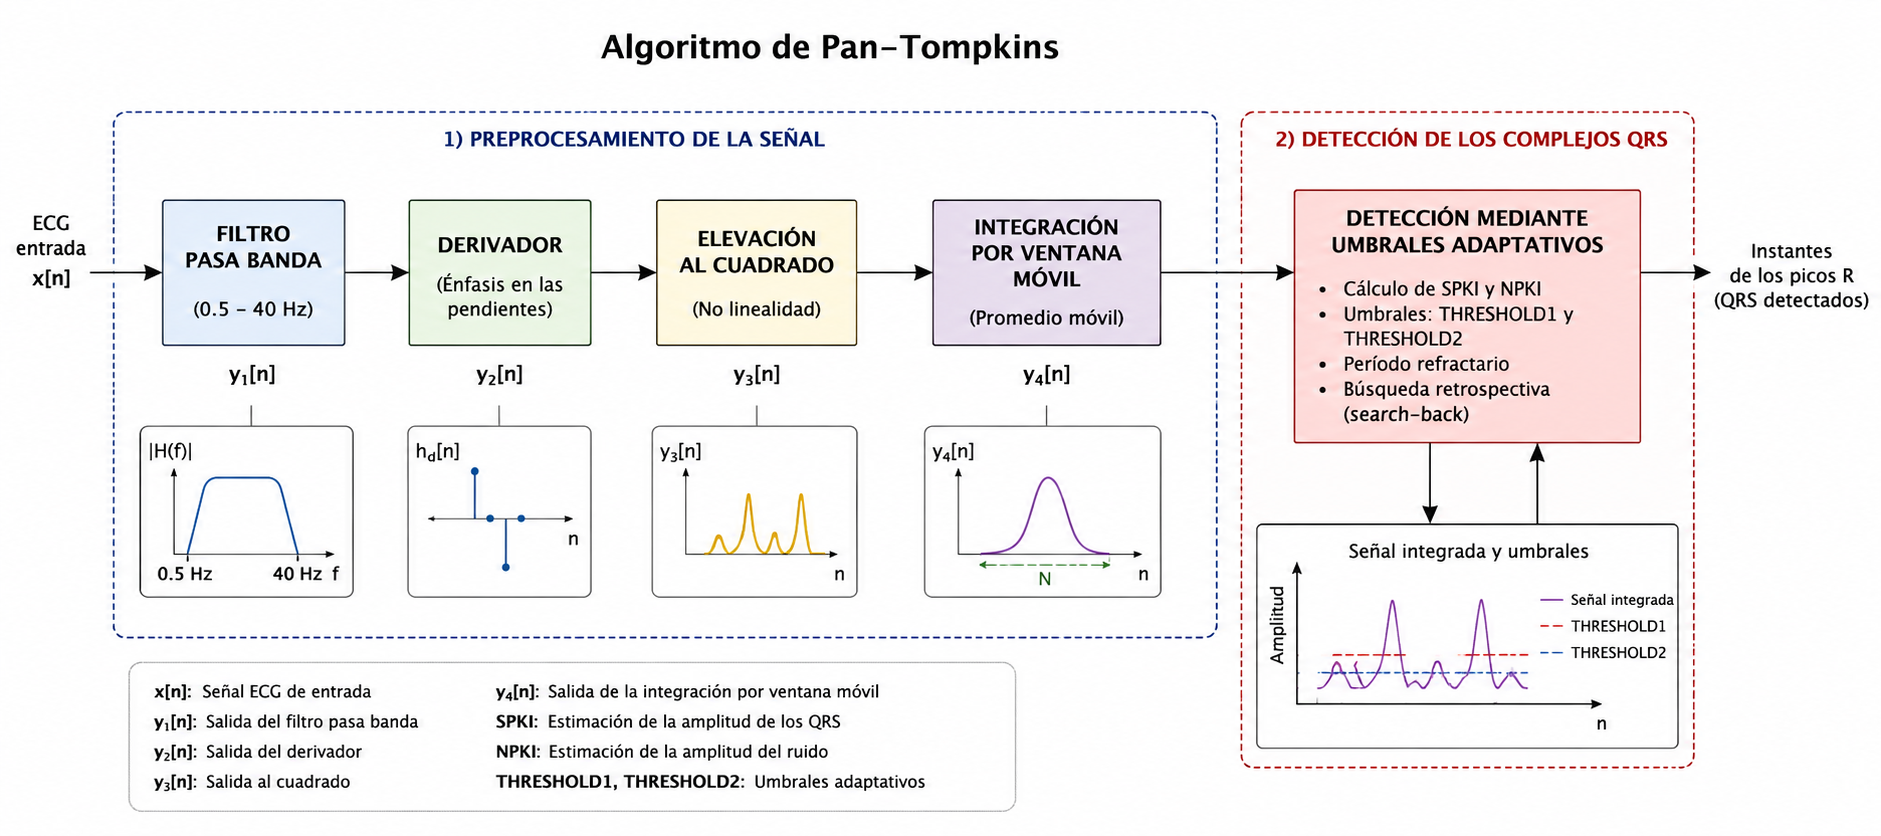
\includegraphics[width=1\textwidth]{imagenes/pan_tompkins_diagrama.png}
					\caption{Diagrama simplificado del algoritmo de Pan--Tompkins.}
					\label{fig:pan_tompkins}
				\end{figure}
 
			\subsection{Etapas de procesamiento de la señal}

				El algoritmo de Pan--Tompkins realiza una serie de operaciones sucesivas sobre la señal ECG con el objetivo de resaltar las características asociadas al complejo QRS. Estas etapas no buscan detectar directamente el latido, sino transformar la señal original en una nueva representación donde los complejos QRS sean más fáciles de identificar y se encuentren mejor diferenciados del ruido, de la línea base y de las ondas P y T.

				El procesamiento aplicado puede representarse como una cadena de bloques compuesta por un filtrado pasa banda, una etapa derivativa, una operación de elevación al cuadrado y una integración mediante ventana móvil. Cada bloque cumple una función específica dentro del acondicionamiento de la señal.

				\subsubsection{Filtro pasa banda}

				La primera etapa del algoritmo consiste en aplicar un filtro pasa banda a la señal ECG de entrada. El objetivo de este bloque es atenuar las componentes de frecuencia que no aportan información relevante para la detección del complejo QRS.

				En señales ECG reales pueden aparecer distintas fuentes de interferencia. Las componentes de muy baja frecuencia suelen estar asociadas a desplazamientos de la línea base, respiración o movimiento de los electrodos. Por otro lado, las componentes de alta frecuencia pueden deberse a ruido muscular, interferencias electromagnéticas o ruido propio del sistema de adquisición.

				El complejo QRS posee un contenido frecuencial característico, asociado a su corta duración temporal y a sus pendientes pronunciadas. Por esta razón, al aplicar un filtro pasa banda se busca conservar principalmente la banda donde se concentra la energía del QRS, reduciendo al mismo tiempo las componentes lentas de la señal y el ruido de alta frecuencia.

				En términos generales, la salida de esta etapa puede expresarse como:

				\begin{equation}
					y_1[n] = H_{PB}\{x[n]\}
				\end{equation}

				donde $x[n]$ es la señal ECG de entrada, $H_{PB}\{\cdot\}$ representa la operación de filtrado pasa banda y $y_1[n]$ es la señal filtrada. Esta señal conserva mejor las componentes asociadas al complejo QRS y constituye la entrada de la etapa derivativa.

				\subsubsection{Etapa derivativa}

				Luego del filtrado pasa banda, se aplica una etapa derivativa. Esta operación permite resaltar los cambios rápidos de la señal, es decir, las pendientes pronunciadas que caracterizan al complejo QRS.

				A diferencia de las ondas P y T, que presentan variaciones más lentas y suaves, el complejo QRS posee una transición rápida en un intervalo temporal reducido. Por este motivo, la derivada tiende a generar valores elevados durante la aparición del QRS y valores menores en las regiones de variación lenta.

				Una aproximación discreta de la derivada puede expresarse de forma general como:

				\begin{equation}
					y_2[n] = \frac{1}{T_s}\left(y_1[n] - y_1[n-1]\right)
				\end{equation}

				donde $T_s$ es el período de muestreo. En implementaciones prácticas pueden utilizarse operadores derivados de varias muestras para mejorar la respuesta frente al ruido y obtener una estimación más robusta de la pendiente.

				La salida $y_2[n]$ contiene información relacionada con la tasa de cambio de la señal filtrada, por lo que permite reforzar la presencia del complejo QRS frente a otras componentes del ECG.

				\subsubsection{Elevación al cuadrado}

				La siguiente etapa consiste en elevar al cuadrado cada muestra de la señal derivada. Esta operación cumple dos funciones principales. En primer lugar, convierte todos los valores de la señal en positivos, eliminando la dependencia del signo de la pendiente. En segundo lugar, amplifica de manera no lineal los valores de mayor amplitud, resaltando aún más las regiones donde la señal presenta cambios bruscos.

				La operación se define como:

				\begin{equation}
					y_3[n] = \left(y_2[n]\right)^2
				\end{equation}

				Como resultado, las pendientes pronunciadas asociadas al complejo QRS generan picos de gran amplitud, mientras que las variaciones pequeñas producidas por ruido o por componentes más lentas quedan relativamente atenuadas. Esta etapa mejora el contraste entre los complejos QRS y el resto de la señal.

				\subsubsection{Integración por ventana móvil}

				Luego de la elevación al cuadrado, se aplica una integración mediante ventana móvil. Esta etapa calcula un promedio de la energía de la señal dentro de una ventana temporal de longitud finita. Su objetivo es combinar la información de amplitud y duración del complejo QRS, generando una señal suavizada donde cada complejo aparece como un pulso ancho y fácilmente detectable.

				La integración por ventana móvil puede expresarse como:

				\begin{equation}
					y_4[n] = \frac{1}{N}\sum_{k=0}^{N-1} y_3[n-k]
				\end{equation}

				donde $N$ es la cantidad de muestras de la ventana de integración. La elección de $N$ está relacionada con la duración esperada del complejo QRS. Si la ventana es demasiado corta, la salida puede fragmentar el complejo en varios picos. En cambio, si la ventana es demasiado larga, se pierde resolución temporal y pueden mezclarse eventos cercanos.

				La salida $y_4[n]$ representa una envolvente de energía de la señal procesada. Sobre esta señal se aplican posteriormente los criterios de detección, ya que los complejos QRS quedan representados como máximos locales claramente diferenciados.






	\section{Placa de Desarrollo}

		\subsection{Microcontrolador STM32F446RE} 

		El sistema fue implementado sobre la placa de desarrollo NUCLEO-F446RE, basada en el microcontrolador STM32F446RE de STMicroelectronics. Este dispositivo incorpora un núcleo ARM Cortex-M4 con unidad de punto flotante (FPU), permitiendo ejecutar algoritmos de procesamiento digital de señales en tiempo real con alta eficiencia.

		Las principales características utilizadas en este proyecto son:

		\begin{itemize}
			\item Núcleo ARM Cortex-M4 con soporte para operaciones en punto flotante de precisión simple (FPU).
			\item Frecuencia de operación de hasta 180 MHz.
			\item 512 KB de memoria Flash.
			\item 128 KB de memoria SRAM.
			\item Dos convertidores analógico-digitales (ADC) de 12 bits.
			\item Convertidor digital-analógico (DAC) de dos canales y 12 bits.
			\item Controlador DMA para transferencia automática de datos.
			\item Temporizadores de propósito general para sincronización del sistema.
		\end{itemize}

		La disponibilidad de una FPU permite implementar el algoritmo de Pan--Tompkins utilizando aritmética en punto flotante, simplificando el desarrollo del software y evitando los errores de cuantización asociados a implementaciones en punto fijo.

		\subsection{Convertidores Analógico-Digitales (ADC1 y ADC2)}

		El sistema utiliza ambos convertidores analógico-digitales disponibles en el microcontrolador.

		\begin{itemize}
			\item Resolución: 12 bits.
			\item Rango de conversión: 0 a 3.3 V.
			\item Frecuencia de muestreo: 200 Hz.
			\item Disparo simultáneo mediante la señal TRGO del temporizador TIM2.
			\item Transferencia mediante DMA en modo circular.
			\item Buffer de adquisición de 64 muestras dividido en dos bloques de 32 muestras.
		\end{itemize}

		ADC1 adquiere la señal ECG principal, mientras que ADC2 permite adquirir una segunda señal utilizada como referencia durante la etapa de cancelación adaptativa implementada previamente mediante el filtro LMS. La salida del filtro LMS constituye la entrada del algoritmo de Pan--Tompkins, permitiendo realizar la detección sobre una señal previamente filtrada. El procesamiento por bloques se realiza utilizando un esquema de doble buffer, donde mientras una mitad del buffer continúa siendo llenada por el DMA, la otra mitad es procesada por el microcontrolador.

		Las muestras adquiridas se normalizan al rango $[-1,1]$ mediante

		\[
		x(n)=\frac{\mathrm{ADC}(n)-2048}{2047.5}.
		\]

		\subsection{Convertidor Digital-Analógico (DAC)}

		El convertidor digital-analógico se emplea para visualizar en tiempo real las distintas señales generadas durante el procesamiento.

		\begin{itemize}
			\item Resolución: 12 bits.
			\item Dos canales de salida.
			\item Actualización sincronizada mediante TIM2.
			\item Transferencia de datos mediante DMA en modo circular.
		\end{itemize}

		El canal DAC1 reproduce continuamente la salida de la etapa de integración por ventana móvil, correspondiente a la señal utilizada posteriormente para la detección de los complejos QRS. El canal DAC2 permite visualizar distintas señales internas del algoritmo, tales como la salida del filtro LMS, la señal adquirida por los ADC, la salida del filtro pasa banda, la señal derivada o la salida del integrador de ventana móvil, seleccionables mediante un pulsador.

		La conversión desde punto flotante al formato de 12 bits del DAC se realiza mediante

		\[
		DAC(n)=\left\lfloor\left(f(n)+1\right)\frac{4095}{2}+0.5\right\rfloor
		\]

		limitando posteriormente el resultado al rango comprendido entre 0 y 4095.

		\subsection{Temporizador TIM2}

		El temporizador TIM2 constituye la referencia temporal de todo el sistema de adquisición y procesamiento.

		\begin{itemize}
			\item Temporizador de propósito general de 32 bits.
			\item Frecuencia de actualización de 200 Hz.
			\item Generación de la señal TRGO utilizada para sincronizar simultáneamente ADC y DAC.
		\end{itemize}

		De esta manera, todas las conversiones analógicas y las actualizaciones de las salidas ocurren de forma perfectamente sincronizada, garantizando un funcionamiento determinístico del sistema de procesamiento en tiempo real.

		\subsection{Acceso Directo a Memoria (DMA)}

		La transferencia de datos entre los periféricos y la memoria se realiza mediante el controlador DMA.

		\begin{itemize}
			\item Transferencia ADC1 $\rightarrow$ memoria.
			\item Transferencia ADC2 $\rightarrow$ memoria.
			\item Transferencia memoria $\rightarrow$ DAC1.
			\item Transferencia memoria $\rightarrow$ DAC2.
			\item Modo circular con interrupciones de media transferencia y transferencia completa.
		\end{itemize}

		El empleo del DMA permite que la adquisición y reproducción de señales se realicen sin intervención directa del procesador, reduciendo significativamente la carga computacional y permitiendo que el núcleo Cortex-M4 dedique la mayor parte del tiempo a la ejecución del algoritmo de procesamiento digital. Además, el esquema de doble buffer implementado posibilita procesar un bloque de muestras mientras el siguiente continúa siendo adquirido, garantizando un flujo continuo de datos sin pérdidas de información.
	\section{Arquitectura y Diseño del Sistema}

	\section{Implementación}

	\section{Resultados Experimentales}

	\section{Conclusiones}

\end{document}
